% Options for packages loaded elsewhere
\PassOptionsToPackage{unicode}{hyperref}
\PassOptionsToPackage{hyphens}{url}
%
\documentclass[
  10pt,
]{article}
\usepackage{amsmath,amssymb}
\usepackage{iftex}
\ifPDFTeX
  \usepackage[T1]{fontenc}
  \usepackage[utf8]{inputenc}
  \usepackage{textcomp} % provide euro and other symbols
\else % if luatex or xetex
  \usepackage{unicode-math} % this also loads fontspec
  \defaultfontfeatures{Scale=MatchLowercase}
  \defaultfontfeatures[\rmfamily]{Ligatures=TeX,Scale=1}
\fi
\usepackage{lmodern}
\ifPDFTeX\else
  % xetex/luatex font selection
  \setmainfont[]{DejaVu Serif}
  \setmonofont[]{DejaVu Sans Mono}
\fi
% Use upquote if available, for straight quotes in verbatim environments
\IfFileExists{upquote.sty}{\usepackage{upquote}}{}
\IfFileExists{microtype.sty}{% use microtype if available
  \usepackage[]{microtype}
  \UseMicrotypeSet[protrusion]{basicmath} % disable protrusion for tt fonts
}{}
\makeatletter
\@ifundefined{KOMAClassName}{% if non-KOMA class
  \IfFileExists{parskip.sty}{%
    \usepackage{parskip}
  }{% else
    \setlength{\parindent}{0pt}
    \setlength{\parskip}{6pt plus 2pt minus 1pt}}
}{% if KOMA class
  \KOMAoptions{parskip=half}}
\makeatother
\usepackage{xcolor}
\usepackage[margin=0.65in]{geometry}
\usepackage{longtable,booktabs,array}
\usepackage{calc} % for calculating minipage widths
% Correct order of tables after \paragraph or \subparagraph
\usepackage{etoolbox}
\makeatletter
\patchcmd\longtable{\par}{\if@noskipsec\mbox{}\fi\par}{}{}
\makeatother
% Allow footnotes in longtable head/foot
\IfFileExists{footnotehyper.sty}{\usepackage{footnotehyper}}{\usepackage{footnote}}
\makesavenoteenv{longtable}
\usepackage{graphicx}
\makeatletter
\def\maxwidth{\ifdim\Gin@nat@width>\linewidth\linewidth\else\Gin@nat@width\fi}
\def\maxheight{\ifdim\Gin@nat@height>\textheight\textheight\else\Gin@nat@height\fi}
\makeatother
% Scale images if necessary, so that they will not overflow the page
% margins by default, and it is still possible to overwrite the defaults
% using explicit options in \includegraphics[width, height, ...]{}
\setkeys{Gin}{width=\maxwidth,height=\maxheight,keepaspectratio}
% Set default figure placement to htbp
\makeatletter
\def\fps@figure{htbp}
\makeatother
\setlength{\emergencystretch}{3em} % prevent overfull lines
\providecommand{\tightlist}{%
  \setlength{\itemsep}{0pt}\setlength{\parskip}{0pt}}
\setcounter{secnumdepth}{-\maxdimen} % remove section numbering
\emergencystretch=3em
\sloppy
\ifLuaTeX
  \usepackage{selnolig}  % disable illegal ligatures
\fi
\usepackage{bookmark}
\IfFileExists{xurl.sty}{\usepackage{xurl}}{} % add URL line breaks if available
\urlstyle{same}
\hypersetup{
  hidelinks,
  pdfcreator={LaTeX via pandoc}}

\author{}
\date{}

\begin{document}

\section{E00 polynomial preflight: actual
result}\label{e00-polynomial-preflight-actual-result}

Date: 2026-10-21. Source/protocol freeze:
\href{https://github.com/aburan28/crypto/commit/66f2d617cc60160b7fece7a38759ca2c61f0bae2}{66f2d617cc60160b7fece7a38759ca2c61f0bae2}.

\textbf{Observed:} five compiled polynomial identities passed exact
integer-coefficient comparison and the repository evaluated-certificate
checks. All five false right-side-plus-one variants were rejected by
both arithmetic paths. The separate supporting certificate/hash suite
passed 22 tests. This is a correctness preflight, not a curve,
subgroup-transfer, solver or performance result.

\subsection{Evidence}\label{evidence}

\begin{itemize}
\tightlist
\item
  \href{run-20261021T144610Z/RECEIPT.json}{Receipt},
  \href{run-20261021T144610Z/issue.json}{issuance output},
  \href{run-20261021T144610Z/check.json}{fresh check output}.
\item
  \href{run-20261021T144610Z/unit-tests.stdout}{Unit-test output},
  \href{run-20261021T144610Z/compiler.txt}{compiler},
  \href{run-20261021T144610Z/host.txt}{host}, and stdout/stderr for
  every command are kept beside the receipt. All recorded commands
  exited 0.
\item
  \href{../E00_PROTOCOL.md}{Frozen protocol} and
  \href{../tools/src/main.rs}{Rust source}. The receipt hashes the
  source, protocol, lockfile, binary and imported repository modules.
\item
  Correctness-only L0 run; no algorithm timing or performance cost was
  measured.
\end{itemize}

\begin{longtable}[]{@{}
  >{\raggedright\arraybackslash}p{(\columnwidth - 8\tabcolsep) * \real{0.1765}}
  >{\raggedleft\arraybackslash}p{(\columnwidth - 8\tabcolsep) * \real{0.2353}}
  >{\raggedleft\arraybackslash}p{(\columnwidth - 8\tabcolsep) * \real{0.2353}}
  >{\raggedright\arraybackslash}p{(\columnwidth - 8\tabcolsep) * \real{0.1765}}
  >{\raggedright\arraybackslash}p{(\columnwidth - 8\tabcolsep) * \real{0.1765}}@{}}
\toprule\noalign{}
\begin{minipage}[b]{\linewidth}\raggedright
Statement
\end{minipage} & \begin{minipage}[b]{\linewidth}\raggedleft
Degree
\end{minipage} & \begin{minipage}[b]{\linewidth}\raggedleft
Expanded terms
\end{minipage} & \begin{minipage}[b]{\linewidth}\raggedright
Exact comparison
\end{minipage} & \begin{minipage}[b]{\linewidth}\raggedright
False variant
\end{minipage} \\
\midrule\noalign{}
\endhead
\bottomrule\noalign{}
\endlastfoot
Trace quartic & 4 & 5 & passed & rejected \\
Chord division & 4 & 9 & passed & rejected \\
Complement A & 4 & 3 & passed & rejected \\
Complement B & 6 & 5 & passed & rejected \\
Model conversion & 9 & 31 & passed & rejected \\
\end{longtable}

Evaluated certificates (32 issuer points plus 32 additional checker
points each):

\begin{itemize}
\tightlist
\item
  Trace quartic:
  \href{run-20261021T144610Z/certificates/trace_quartic_discriminant.json}{IDC1h4275fa8068385ce3}.
\item
  Chord division:
  \href{run-20261021T144610Z/certificates/trace_chord_polynomial_division.json}{IDC1h57c015780fe88055}.
\item
  Complement A:
  \href{run-20261021T144610Z/certificates/cover_complement_A_cleared.json}{IDC1h30c6f3a4043fe787}.
\item
  Complement B:
  \href{run-20261021T144610Z/certificates/cover_complement_B_cleared.json}{IDC1hdf7545f3ee4dca7c}.
\item
  Model conversion:
  \href{run-20261021T144610Z/certificates/cover_complement_change_of_variables.json}{IDC1h9293014287b4205c}.
\end{itemize}

The term counts describe symbolic expressions, not algorithm operation
counts or useful relations. The 32 additional points use the checker's
domain-separated stream. They are not an independent-host replay, and
the certificates have proof=null. Published records were also checked to
have 32 issuer points, seed 20261021 and proof=null.

\subsection{What this changes}\label{what-this-changes}

The concrete trace-quartic and cover-complement designs have
reproducible arithmetic preconditions. E01--E17 now have specific
questions, families, controls, falsifiers and dependencies in the
\href{../EXPERIMENTS.md}{experiment program}. No point census,
restricted-base relation experiment, Groebner comparison, cover search,
Jacobian transfer, pipeline ablation or NIST-size execution has been
performed here.

\subsection{Remaining obligations}\label{remaining-obligations}

Formal Lean proofs were not compiled: lake/Lean are unavailable in this
environment. Exact coefficient matching is an implementation check, not
a replacement for the group's geometric hypotheses, rational-map
exceptional charts or formal bridge. Independent-host replay remains
pending. The original three route cards remain blocked on their actual
point/solver/transfer implementations and admitted fixture/cost
protocols.

\subsection{Visual and canonical
views}\label{visual-and-canonical-views}

\begin{figure}
\centering
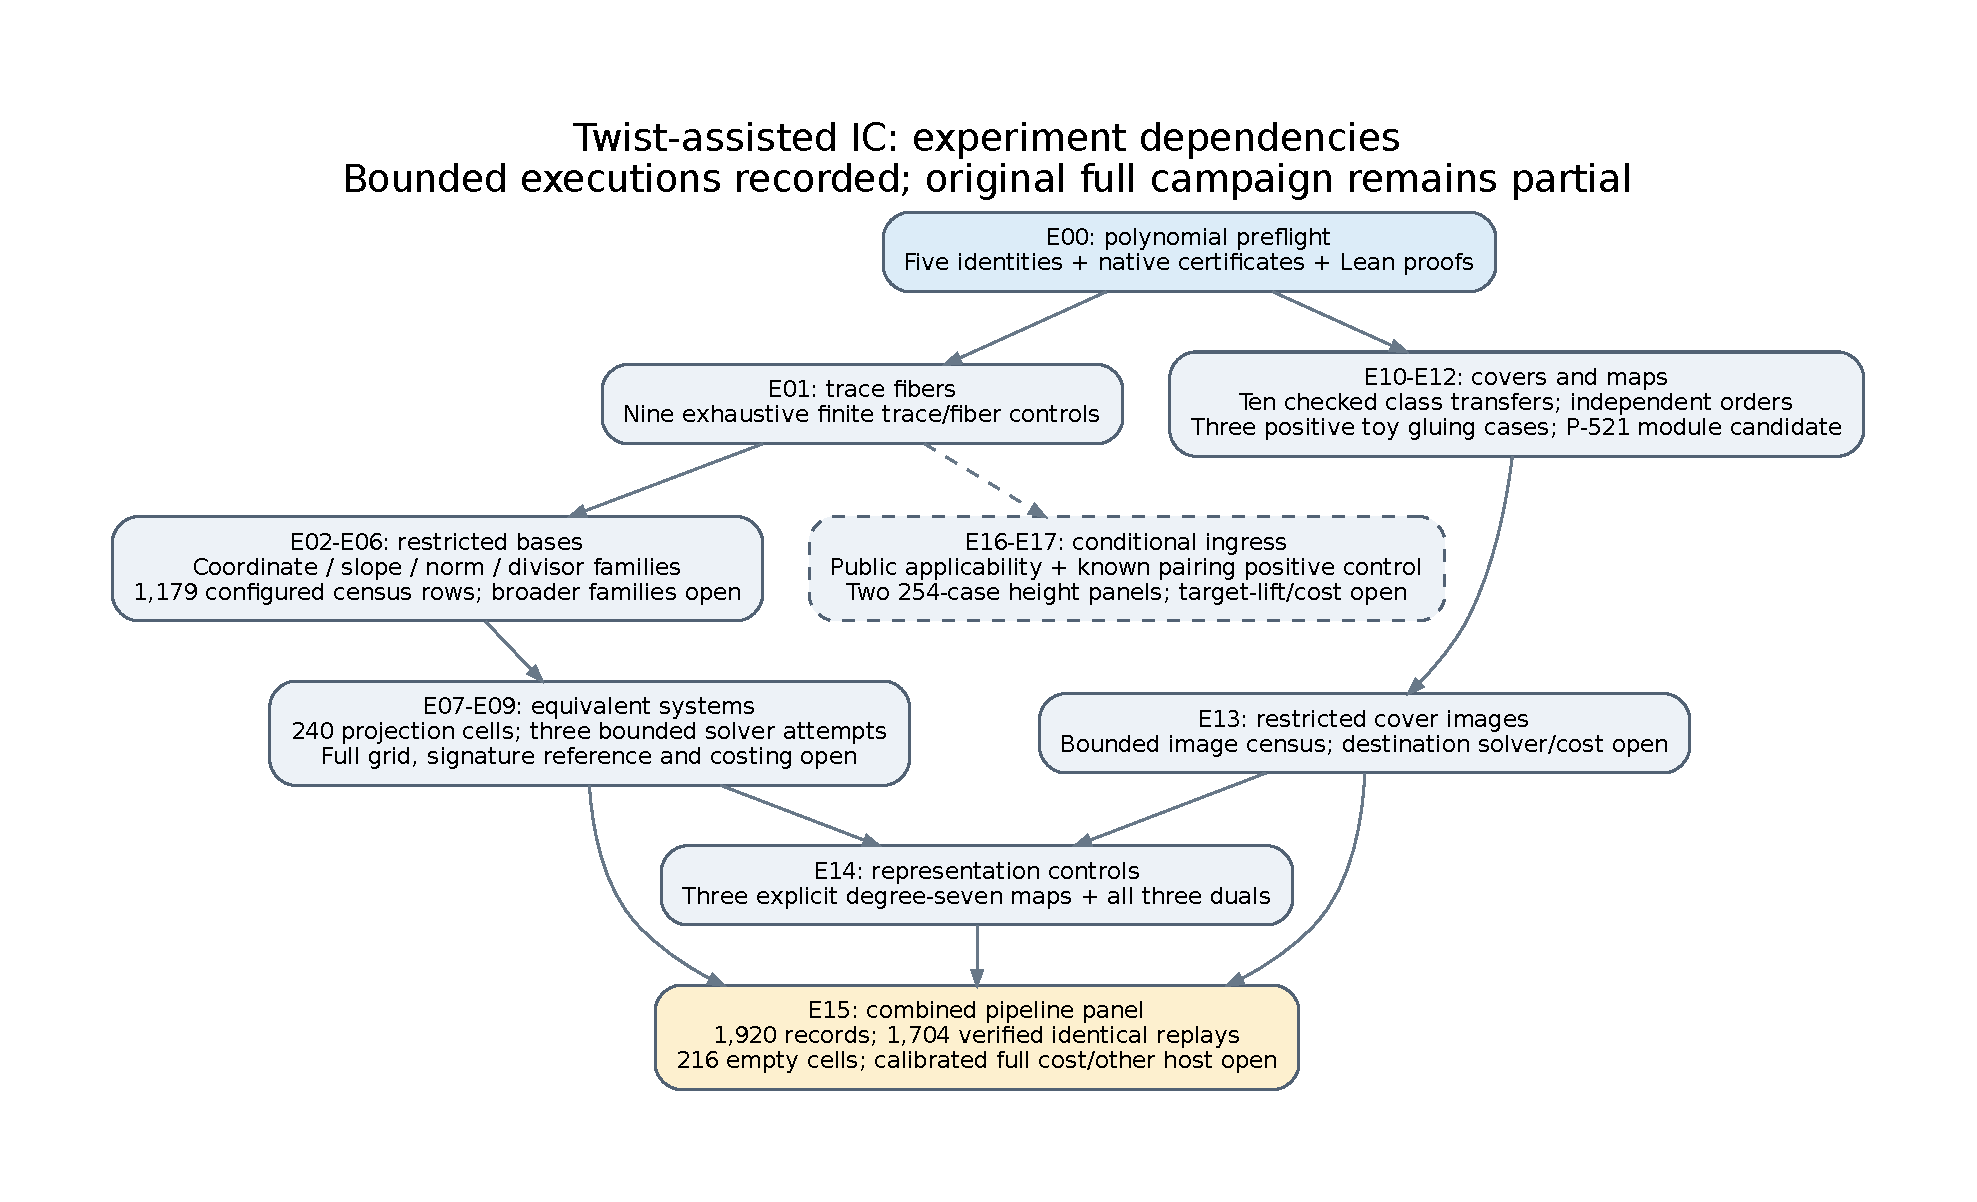
\includegraphics{../PROGRAM.pdf}
\caption{Experiment dependencies; E01--E17 are planned, not results}
\end{figure}

The \href{../PROGRAM.dot}{editable diagram} and
\href{../PROGRAM.svg}{SVG} describe dependencies. There are no
comparable performance values to graph. This result adds no IC/rho
ratio, curve registration, method/session or measured leaderboard row;
the scoreboard, progress timeline, leaderboard and browser therefore
receive no new value from it.

Individual certificate/receipt paths are linked directly and stay as
loose immutable artifacts; they are not repacked. Later checks use fresh
output directories.

\end{document}
